\documentclass{standalone}
\usepackage{tikz}
\usetikzlibrary{patterns, positioning}
\usepackage[sfdefault]{ClearSans} %% option 'sfdefault' activates Clear Sans as the default text font
\usepackage[T1]{fontenc}

\begin{document}
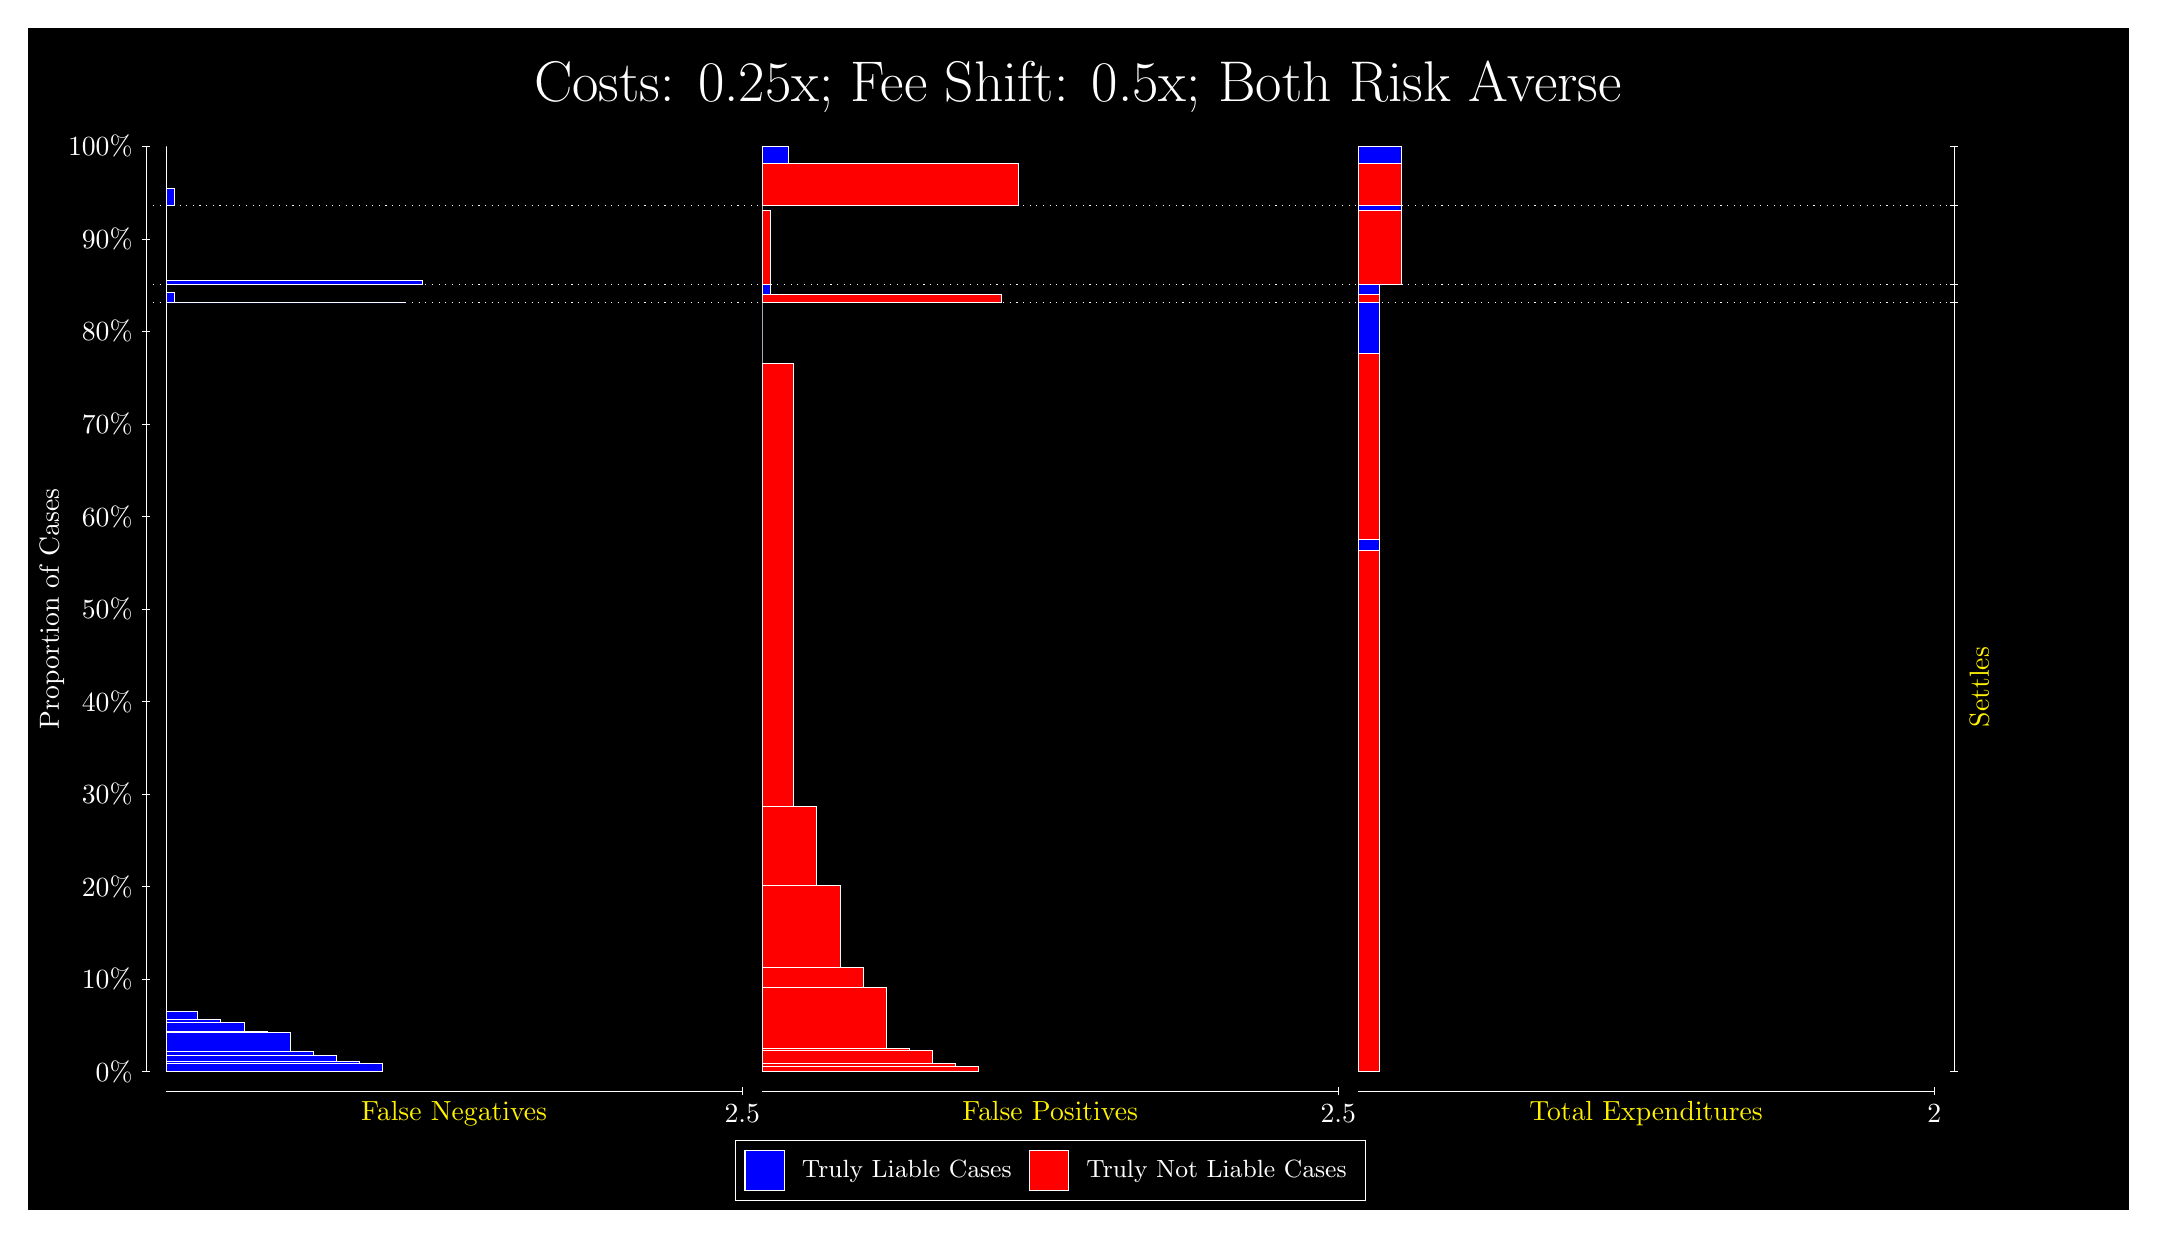
\begin{tikzpicture}
\draw[fill=black] (0,0) rectangle (26.667,15);
\draw[text=white] (0,13.5) rectangle (26.667,15) node[midway] {\huge Costs: 0.25x; Fee Shift: 0.5x; Both Risk Averse};
\draw[white, very thin] (1.5,1.75) -- (1.5,13.5);
\node[rotate=90, text=white, anchor=center] at (0.3, 7.625) {Proportion of Cases};
\draw[white, very thin] (1.45,1.75) -- (1.55,1.75);
\node[text=white, anchor=east] at (1.45, 1.75) {0\%};
\draw[white, very thin] (1.45,2.925) -- (1.55,2.925);
\node[text=white, anchor=east] at (1.45, 2.925) {10\%};
\draw[white, very thin] (1.45,4.1) -- (1.55,4.1);
\node[text=white, anchor=east] at (1.45, 4.1) {20\%};
\draw[white, very thin] (1.45,5.275) -- (1.55,5.275);
\node[text=white, anchor=east] at (1.45, 5.275) {30\%};
\draw[white, very thin] (1.45,6.45) -- (1.55,6.45);
\node[text=white, anchor=east] at (1.45, 6.45) {40\%};
\draw[white, very thin] (1.45,7.625) -- (1.55,7.625);
\node[text=white, anchor=east] at (1.45, 7.625) {50\%};
\draw[white, very thin] (1.45,8.8) -- (1.55,8.8);
\node[text=white, anchor=east] at (1.45, 8.8) {60\%};
\draw[white, very thin] (1.45,9.975) -- (1.55,9.975);
\node[text=white, anchor=east] at (1.45, 9.975) {70\%};
\draw[white, very thin] (1.45,11.15) -- (1.55,11.15);
\node[text=white, anchor=east] at (1.45, 11.15) {80\%};
\draw[white, very thin] (1.45,12.325) -- (1.55,12.325);
\node[text=white, anchor=east] at (1.45, 12.325) {90\%};
\draw[white, very thin] (1.45,13.5) -- (1.55,13.5);
\node[text=white, anchor=east] at (1.45, 13.5) {100\%};

\draw[white, very thin] (24.457,1.75) -- (24.457,13.5);
\draw[white, very thin] (24.407,1.75) -- (24.507,1.75);
\node[anchor=west] at (24.407, 1.75) {};
\draw[white, very thin] (24.407,11.514) -- (24.507,11.514);
\node[anchor=west] at (24.407, 11.514) {};
\draw[white, very thin] (24.407,11.521) -- (24.507,11.521);
\node[anchor=west] at (24.407, 11.521) {};
\draw[white, very thin] (24.407,11.743) -- (24.507,11.743);
\node[anchor=west] at (24.407, 11.743) {};
\draw[white, very thin] (24.407,12.752) -- (24.507,12.752);
\node[anchor=west] at (24.407, 12.752) {};
\draw[white, very thin] (24.407,13.5) -- (24.507,13.5);
\node[anchor=west] at (24.407, 13.5) {};

\draw[white, very thin, fill=blue] (1.75,1.75) rectangle (4.4946,1.8548);
\draw[white, very thin, fill=blue] (1.75,1.8548) rectangle (4.2018,1.8832);
\draw[white, very thin, fill=blue] (1.75,1.8832) rectangle (3.9091,1.9589);
\draw[white, very thin, fill=blue] (1.75,1.9589) rectangle (3.6163,2.0032);
\draw[white, very thin, fill=blue] (1.75,2.0032) rectangle (3.3236,2.2454);
\draw[white, very thin, fill=blue] (1.75,2.2454) rectangle (3.0308,2.2609);
\draw[white, very thin, fill=blue] (1.75,2.2609) rectangle (2.738,2.3818);
\draw[white, very thin, fill=blue] (1.75,2.3818) rectangle (2.4453,2.4178);
\draw[white, very thin, fill=blue] (1.75,2.4178) rectangle (2.1525,2.5204);
\draw[white, very thin, fill=red] (1.75,2.5204) rectangle (1.75,11.514);
\draw[white, very thin, fill=blue] (1.75,11.514) rectangle (4.7873,11.514);
\draw[white, very thin, fill=red] (1.75,11.514) rectangle (1.75,11.521);
\draw[white, very thin, fill=blue] (1.75,11.521) rectangle (1.8598,11.646);
\draw[white, very thin, fill=red] (1.75,11.646) rectangle (1.75,11.743);
\draw[white, very thin, fill=blue] (1.75,11.743) rectangle (5.0069,11.801);
\draw[white, very thin, fill=red] (1.75,11.801) rectangle (1.75,12.752);
\draw[white, very thin, fill=blue] (1.75,12.752) rectangle (1.8598,12.973);
\draw[white, very thin, fill=red] (1.75,12.973) rectangle (1.75,13.5);
\draw[white, very thin, fill=red] (9.3189,1.75) rectangle (12.063,1.8215);
\draw[white, very thin, fill=red] (9.3189,1.8215) rectangle (11.771,1.8566);
\draw[white, very thin, fill=red] (9.3189,1.8566) rectangle (11.478,2.0146);
\draw[white, very thin, fill=red] (9.3189,2.0146) rectangle (11.185,2.044);
\draw[white, very thin, fill=red] (9.3189,2.044) rectangle (10.892,2.8185);
\draw[white, very thin, fill=red] (9.3189,2.8185) rectangle (10.6,3.0728);
\draw[white, very thin, fill=red] (9.3189,3.0728) rectangle (10.307,4.1187);
\draw[white, very thin, fill=red] (9.3189,4.1187) rectangle (10.014,5.1249);
\draw[white, very thin, fill=red] (9.3189,5.1249) rectangle (9.7214,10.744);
\draw[white, very thin, fill=blue] (9.3189,10.744) rectangle (9.3189,11.514);
\draw[white, very thin, fill=red] (9.3189,11.514) rectangle (9.4287,11.521);
\draw[white, very thin, fill=blue] (9.3189,11.521) rectangle (9.3189,11.521);
\draw[white, very thin, fill=red] (9.3189,11.521) rectangle (12.356,11.618);
\draw[white, very thin, fill=blue] (9.3189,11.618) rectangle (9.4287,11.743);
\draw[white, very thin, fill=red] (9.3189,11.743) rectangle (9.4287,12.694);
\draw[white, very thin, fill=blue] (9.3189,12.694) rectangle (9.3189,12.752);
\draw[white, very thin, fill=red] (9.3189,12.752) rectangle (12.576,13.279);
\draw[white, very thin, fill=blue] (9.3189,13.279) rectangle (9.6482,13.5);
\draw[white, very thin, fill=red] (16.888,1.75) rectangle (17.162,8.3749);
\draw[white, very thin, fill=blue] (16.888,8.3749) rectangle (17.162,8.5081);
\draw[white, very thin, fill=red] (16.888,8.5081) rectangle (17.162,10.877);
\draw[white, very thin, fill=blue] (16.888,10.877) rectangle (17.162,11.514);
\draw[white, very thin, fill=red] (16.888,11.514) rectangle (17.162,11.521);
\draw[white, very thin, fill=blue] (16.888,11.521) rectangle (17.162,11.521);
\draw[white, very thin, fill=red] (16.888,11.521) rectangle (17.162,11.618);
\draw[white, very thin, fill=blue] (16.888,11.618) rectangle (17.162,11.743);
\draw[white, very thin, fill=red] (16.888,11.743) rectangle (17.437,12.694);
\draw[white, very thin, fill=blue] (16.888,12.694) rectangle (17.437,12.752);
\draw[white, very thin, fill=red] (16.888,12.752) rectangle (17.437,13.279);
\draw[white, very thin, fill=blue] (16.888,13.279) rectangle (17.437,13.5);
\draw[white, dotted] (1.5,11.514) -- (24.457,11.514);
\draw[white, dotted] (1.5,11.521) -- (24.457,11.521);
\draw[white, dotted] (1.5,11.743) -- (24.457,11.743);
\draw[white, dotted] (1.5,12.752) -- (24.457,12.752);
\draw[white, very thin] (1.75,1.5) -- (9.0689,1.5);
\node[text=yellow, anchor=north] at (5.4094, 1.5) {False Negatives};
\draw[white, very thin] (9.0689,1.45) -- (9.0689,1.55);
\node[text=white, anchor=north] at (9.0689, 1.45) {2.5};

\draw[white, very thin] (9.3189,1.5) -- (16.638,1.5);
\node[text=yellow, anchor=north] at (12.978, 1.5) {False Positives};
\draw[white, very thin] (16.638,1.45) -- (16.638,1.55);
\node[text=white, anchor=north] at (16.638, 1.45) {2.5};

\draw[white, very thin] (16.888,1.5) -- (24.207,1.5);
\node[text=yellow, anchor=north] at (20.547, 1.5) {Total Expenditures};
\draw[white, very thin] (24.207,1.45) -- (24.207,1.55);
\node[text=white, anchor=north] at (24.207, 1.45) {2};

\node[text=yellow, centered, rotate=90] at (24.777, 6.632) {Settles};





\draw (12.978300999999998,1.5) node[draw=none] (baseCoordinate) {};
\begin{scope}[align=center]
        \matrix[scale=0.5, draw=white, below=0.5cm of baseCoordinate, nodes={draw}, column sep=0.1cm]{
            \node[rectangle, draw, minimum width=0.5cm, minimum height=0.5cm, fill=blue] {}; &
            \node[draw=none, font=\small, text=white] (B) {Truly Liable Cases}; &
            \node[rectangle, draw, minimum width=0.5cm, minimum height=0.5cm, fill=red] {}; &
            \node[draw=none, font=\small, text=white] (B) {Truly Not Liable Cases}; \\
            };
\end{scope}

\end{tikzpicture}
\end{document}